\documentclass[11pt]{article}

\usepackage[a4paper,margin=1in]{geometry}
\usepackage{amsmath}
\usepackage{amssymb}
\usepackage{booktabs}
\usepackage{tabularx}
\usepackage{graphicx}
\usepackage[hidelinks]{hyperref}
\usepackage[authoryear,round]{natbib}
\usepackage{siunitx}
\usepackage{tikz}
\usetikzlibrary{arrows.meta,positioning}
\sisetup{group-separator={,}, group-minimum-digits=4}

\graphicspath{{assets/}}

\title{Computational Pathology and Benchmark Datasets:\\
An Introduction to the Domain and Data}
\author{Yannik Queisler}
\date{\today}

\begin{document}
\maketitle

\begin{abstract}
\begingroup
\setlength{\emergencystretch}{2em}
\noindent This report introduces the domain of computational pathology and the four public
histopathology datasets it covers. It first explains what diagnostic pathology is, how a stained glass slide becomes a
gigapixel whole-slide image, why such images are tiled into patches, and how weakly supervised and
frozen foundation-model pipelines turn those patches into predictions. It then describes, in detail,
four H\&E datasets --- CAMELYON16, TCGA-UT, BRACS, and PANDA --- presented in the order of the
diagnostic question they pose, from detection (\emph{is cancer present?}) through cancer typing and
lesion subtyping to ordinal grading (\emph{how aggressive is it?}). Each dataset is given with its
clinical background, an example patch, a summary table, and its class distribution.
\par
\endgroup
\end{abstract}

\setcounter{tocdepth}{2}
\tableofcontents
\clearpage

\section{Computational Pathology}
\label{sec:cpath}
Diagnostic pathology is the branch of medicine that examines tissue under the microscope to detect
and characterise disease. When cancer is suspected, a biopsy or surgical resection is fixed, thinly
sectioned, mounted on a glass slide, and stained --- most commonly with hematoxylin and eosin
(H\&E), which colours cell nuclei blue-purple and cytoplasm and stroma shades of pink --- so that a
pathologist can read cellular and tissue morphology and render a diagnosis. This reading is the
clinical reference standard for cancer detection, typing, and grading, and it drives treatment
decisions. It is also labour-intensive, requires scarce expertise, and is subject to inter- and
intra-observer variability, which motivates computational assistance
\citep{madabhushi2016imageAnalysis,song2023aiPathology}.

Computerised analysis of microscopy images is not new: the earliest work on cell and chromosome
image analysis dates back more than fifty years. What changed
recently is scale and method. \emph{Digital pathology} digitises the glass slide with a
whole-slide scanner, enabling telepathology, archiving, and education; \emph{computational
pathology} (CPath) goes further, treating the resulting images as high-dimensional data for
quantitative, reproducible analysis and integrating them with clinical and molecular context. A useful distinction
here is between the \emph{ground truth}, the abstract label one wishes to predict, and the
\emph{gold standard}, the practical benchmark used to approximate it --- typically a pathologist's
own assessment. Because algorithmic outputs can eventually prove more reproducible than the human
benchmark that trained them, CPath must navigate a \emph{gold-standard paradox} in which the
reference itself is imperfect \citep{abels2019computationalPathology,madabhushi2016imageAnalysis,hosseini2024computationalPathology}.

The clinical value of CPath is usually framed along two axes.
\emph{Automation} standardises tasks pathologists already perform --- detecting metastases,
subtyping and grading tumours, quantifying immunohistochemical markers --- reducing workload and
observer variability. \emph{Discovery} identifies signatures beyond human visual limits, such as
predicting prognosis, therapy response, or molecular alterations (for example microsatellite
instability) directly from H\&E morphology; these are the ``sub-visual'' features that quantitative
analysis can mine but a human eye cannot reliably see \citep{song2023aiPathology,madabhushi2016imageAnalysis}.
Table~\ref{tab:cpath-tasks} summarises representative tasks. The datasets in this report all sit
on the automation axis: each carries a diagnostic label a pathologist established, and the task is
to predict it from H\&E tissue.

\begin{table}[ht]
  \centering
  \small
  \begin{tabularx}{\linewidth}{@{}lX@{}}
    \toprule
    Role & Representative tasks\\
    \midrule
    Automation & Metastasis detection; cancer-type classification; tumour subtyping; Gleason/ISUP
                 grading; mitosis counting; immunohistochemistry (PD-L1, Ki-67) quantification\\
    Discovery  & Prognosis and recurrence-risk prediction; molecular-marker prediction (e.g.\
                 microsatellite instability) from H\&E; therapy-response biomarkers\\
    \bottomrule
  \end{tabularx}
  \caption{Two roles of computational pathology, following \citet{song2023aiPathology} and
  \citet{madabhushi2016imageAnalysis}. The datasets in this report are automation tasks with
  pathologist-established labels.}
  \label{tab:cpath-tasks}
\end{table}

\subsection{The whole-slide imaging pipeline}
\label{sec:pipeline}
A digitised slide is a \emph{whole-slide image} (WSI): a single H\&E image of an entire tissue
section, routinely on the order of \num{100000}$\times$\num{100000} pixels and \num{0.5}--\num{4}\,GB
in size. To make this tractable, a WSI is
stored as a \emph{pyramid} of progressively downsampled copies, so the same slide can be read at
several magnifications (Table~\ref{tab:magnification}): high magnification resolves nuclear detail
and mitoses, while lower magnifications carry the tissue-architectural context that diagnosis also
depends on. Scanning the whole section, rather than a manually chosen field of view, removes
selection bias and captures intratumoral heterogeneity, but it produces far more data than fits in
GPU memory \citep{song2023aiPathology,abels2019computationalPathology}.

\begin{table}[ht]
  \centering
  \small
  \begin{tabularx}{\linewidth}{@{}llX@{}}
    \toprule
    Magnification & Resolution & What it resolves\\
    \midrule
    \num{40}$\times$ & ${\approx}\num{0.25}\,\mu$m/pixel & Nuclear detail, chromatin, mitotic figures\\
    \num{20}$\times$ & ${\approx}\num{0.5}\,\mu$m/pixel  & Cellular morphology, individual glands\\
    \num{10}$\times$ & ${\approx}\num{1.0}\,\mu$m/pixel  & Local tissue architecture\\
    \num{5}$\times$  & ${\approx}\num{2.0}\,\mu$m/pixel  & Macro-architectural context\\
    \bottomrule
  \end{tabularx}
  \caption{Typical magnification levels of a pyramidal WSI and the morphology each makes legible
  \citep{song2023aiPathology}. High magnifications are needed for nuclear grading, lower ones for
  architectural context.}
  \label{tab:magnification}
\end{table}

The standard response to the size of a WSI is a divide-and-conquer strategy: the image is
partitioned into small \emph{patches} (also called \emph{tiles}), $256\times256$ pixels to match the
input size of the encoder (Section~\ref{sec:learning}), each processed
independently and later aggregated into a slide- or patient-level prediction
\citep{song2023aiPathology}. Figure~\ref{fig:pipeline} sketches the resulting pipeline, from stained
slide to prediction, that every dataset in this report passes through.

\begin{figure}[ht]
  \centering
  \resizebox{\textwidth}{!}{%
  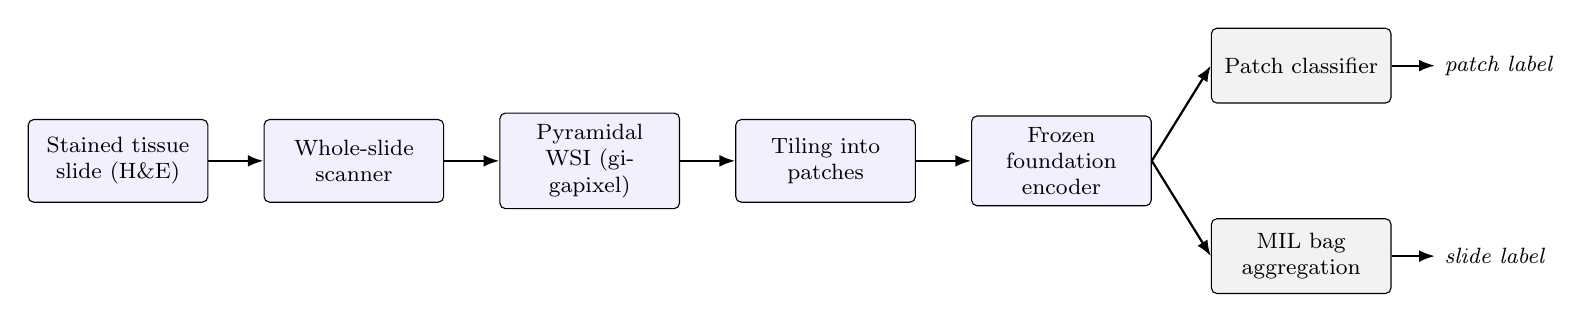
\begin{tikzpicture}[
    node distance=0.55cm and 0.7cm,
    stage/.style={draw, rounded corners=2pt, align=center, fill=blue!6, inner sep=4pt,
                  font=\footnotesize, text width=2.0cm, minimum height=1.05cm},
    head/.style={draw, rounded corners=2pt, align=center, fill=gray!10, inner sep=4pt,
                 font=\footnotesize, text width=2.0cm, minimum height=0.95cm},
    lab/.style={font=\footnotesize\itshape},
    arrow/.style={-{Latex[length=2mm]}, thick}
  ]
    \node[stage] (slide) {Stained tissue slide (H\&E)};
    \node[stage, right=of slide] (scan) {Whole-slide scanner};
    \node[stage, right=of scan] (wsi) {Pyramidal WSI (gigapixel)};
    \node[stage, right=of wsi] (patch) {Tiling into patches};
    \node[stage, right=of patch] (enc) {Frozen foundation encoder};
    \node[head, above right=0.15cm and 0.75cm of enc] (phead) {Patch classifier};
    \node[head, below right=0.15cm and 0.75cm of enc] (mhead) {MIL bag aggregation};
    \node[lab, right=0.55cm of phead] (plabel) {patch label};
    \node[lab, right=0.55cm of mhead] (slabel) {slide label};
    \draw[arrow] (slide)--(scan);
    \draw[arrow] (scan)--(wsi);
    \draw[arrow] (wsi)--(patch);
    \draw[arrow] (patch)--(enc);
    \draw[arrow] (enc.east) -- (phead.west);
    \draw[arrow] (enc.east) -- (mhead.west);
    \draw[arrow] (phead)--(plabel);
    \draw[arrow] (mhead)--(slabel);
  \end{tikzpicture}%
  }
  \caption{The computational-pathology pipeline the datasets pass through. A stained slide is
  scanned into a pyramidal WSI and tiled into patches; a frozen foundation-model encoder embeds each
  patch once, after which either a patch classifier predicts a per-tile label or a multiple-instance
  head aggregates the patch features of a slide into a slide-level prediction.}
  \label{fig:pipeline}
\end{figure}

\subsection{Learning from patches: weak supervision and foundation models}
\label{sec:learning}
How labels attach to these units determines the learning regime. When each patch carries a reliable
label --- because it was cropped from a pathologist-selected region, or intersected with an expert
pixel mask --- ordinary patch classification applies. When only a slide-level diagnosis is
available, the problem is \emph{weakly supervised}: the slide is a \emph{bag} of patch
\emph{instances} that share one label, and \emph{multiple-instance learning} (MIL) aggregates the
instances --- typically through a learned attention mechanism that weights diagnostically salient
patches --- into a slide prediction \citep{song2023aiPathology,hosseini2024computationalPathology}.
Because tiling discards spatial context, context-aware models such as graph neural networks (over
patches or nuclei) and transformers (with global self-attention) are sometimes used to recover it,
but the attention-MIL bag remains the workhorse for slide-level tasks. Both regimes appear in the
datasets below. Only TCGA-UT retains the same target across them; CAMELYON16, BRACS, and PANDA
change the label meaning or granularity between patch and WSI prediction.

The features fed to these heads have shifted from hand-crafted descriptors --- interpretable
measurements of nuclear shape, texture, or spatial architecture --- to learned representations that
capture patterns beyond human perception. Modern CPath rarely trains an image encoder from scratch:
a pathology \emph{foundation model}, pre-trained self-supervised on large slide archives, provides a
frozen feature extractor that embeds each patch once into a fixed-length vector, leaving only a
lightweight classifier or MIL head to train. Virchow2 is one such H\&E foundation model
\citep{vorontsov2024virchow,zimmermann2024virchow2}. Freezing the representation lets a study isolate
the effect of a downstream modelling choice from the confounds of end-to-end backbone training, and
makes the patch and MIL regimes directly comparable, because both consume the same embeddings.

\subsection{Data and annotation}
\label{sec:data-challenge}
Deep learning is data-hungry, and expert annotation is the binding constraint in CPath: pathologist
labelling is slow, expensive, and hard to scale, so datasets range from densely mask-annotated
cohorts to those carrying only a single slide-level diagnosis
\citep{abels2019computationalPathology,hosseini2024computationalPathology}. The four datasets in this
report deliberately span that range of annotation form, from pixel-level tumour masks through
region-of-interest crops to a single slide-level diagnosis. The next section introduces them in the
order of the diagnostic question they pose.

\section{Datasets}
\label{sec:datasets}
Four public H\&E datasets are used, described here in the order of the diagnostic question they
pose --- an arc that also escalates the structure of the label and varies the organ and the form of
annotation:

\begin{itemize}
  \item \textbf{CAMELYON16} --- \emph{is cancer present?} Binary metastasis \emph{detection} in
        sentinel lymph nodes, with pixel-mask annotations.
  \item \textbf{TCGA-UT} --- \emph{what cancer is it?} Pan-cancer \emph{typing} across 32 cancer types,
        each patch labelled with its slide's cancer type.
  \item \textbf{BRACS} --- \emph{how abnormal is this tissue?} Breast-lesion \emph{subtyping} along
        the benign--atypical--malignant continuum, with region-of-interest annotations.
  \item \textbf{PANDA} --- \emph{how aggressive is it?} Ordinal ISUP \emph{grading} of prostate
        biopsies, with region masks and built-in two-provider heterogeneity.
\end{itemize}

\subsection{CAMELYON16 --- lymph-node metastasis detection}
\label{sec:camelyon16}
CAMELYON16 is an organ-specific H\&E cohort of sentinel lymph-node sections for the detection of
breast-cancer metastases \citep{bejnordi2017diagnostic,litjens2018gigascience}. The diagnostic
question is the most basic in oncology --- \emph{is cancer present?} --- and the label is binary:
each slide is either \emph{normal} or contains \emph{tumor} (metastasis). Expert annotations are
supplied as pixel-level masks marking tumour tissue, rather than as cropped regions, so individual
tiles can be labelled by intersecting them with the mask. The slides are tiled once into
non-overlapping $256\times256$ patches at \num{20}x. A patch is kept only if it clears a
tissue-foreground stack --- Otsu thresholding (at least \num{10}\% foreground), a
standard-deviation filter (at least \num{8} gray levels), Canny edge detection, and an isolation
filter that discards patches with fewer than two tissue neighbours. Each surviving patch is
then labelled from the WSI mask: it is tumour when at least \num{50}\% of the aligned mask pixels
have value \num{2}, and normal otherwise.

The benchmark uses \num{398} of the \num{399} published slides (\num{160} tumor, \num{238} normal)
after excluding one slide without usable tile evidence; each slide is its own patient, so
slide-disjoint splits coincide with patient-disjoint splits. Because metastatic tissue occupies only
a small fraction of a sectioned node, mask-derived tumor tiles are scarce: the patch distribution is
\num{3088478} normal against \num{108855} tumor tiles (Table~\ref{tab:camelyon16-summary},
Figure~\ref{fig:camelyon16-dist}), even though tumour and normal slides are themselves close to even
(\num{160} versus \num{238})---tumour tiles are scarce even on slides that do contain a metastasis. The
\num{20} tumor slides whose annotations are not exhaustive are excluded from the tile-labelling
regime, where unannotated tumour could be mislabelled as normal, but retained where only the reliable
slide-level label is used.

\begin{table}[ht]
  \centering
  \begin{minipage}{0.32\linewidth}
    \centering
    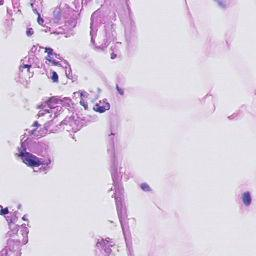
\includegraphics[width=\linewidth]{camelyon16_example_patch.jpg}%
  \end{minipage}
  \hfill
  \begin{minipage}{0.62\linewidth}
    \centering
    \small
    \begin{tabular}{ll}
      \toprule
      Property & Value\\
      \midrule
      WSIs (tumor / normal) & \num{160} / \num{238}\\
      Patch-labelled WSIs & \num{378}\\
      Patch labels & tumor, normal\\
      Eligible patches (tumor / normal) & \num{108855} / \num{3088478}\\
      \bottomrule
    \end{tabular}%
  \end{minipage}
  \caption{CAMELYON16 dataset properties, alongside an example $256\times256$ tumor patch.
  Tumour patches are scarce even within slides that contain a metastasis.}
  \label{tab:camelyon16-summary}
\end{table}

\begin{figure}[ht]
  \centering
  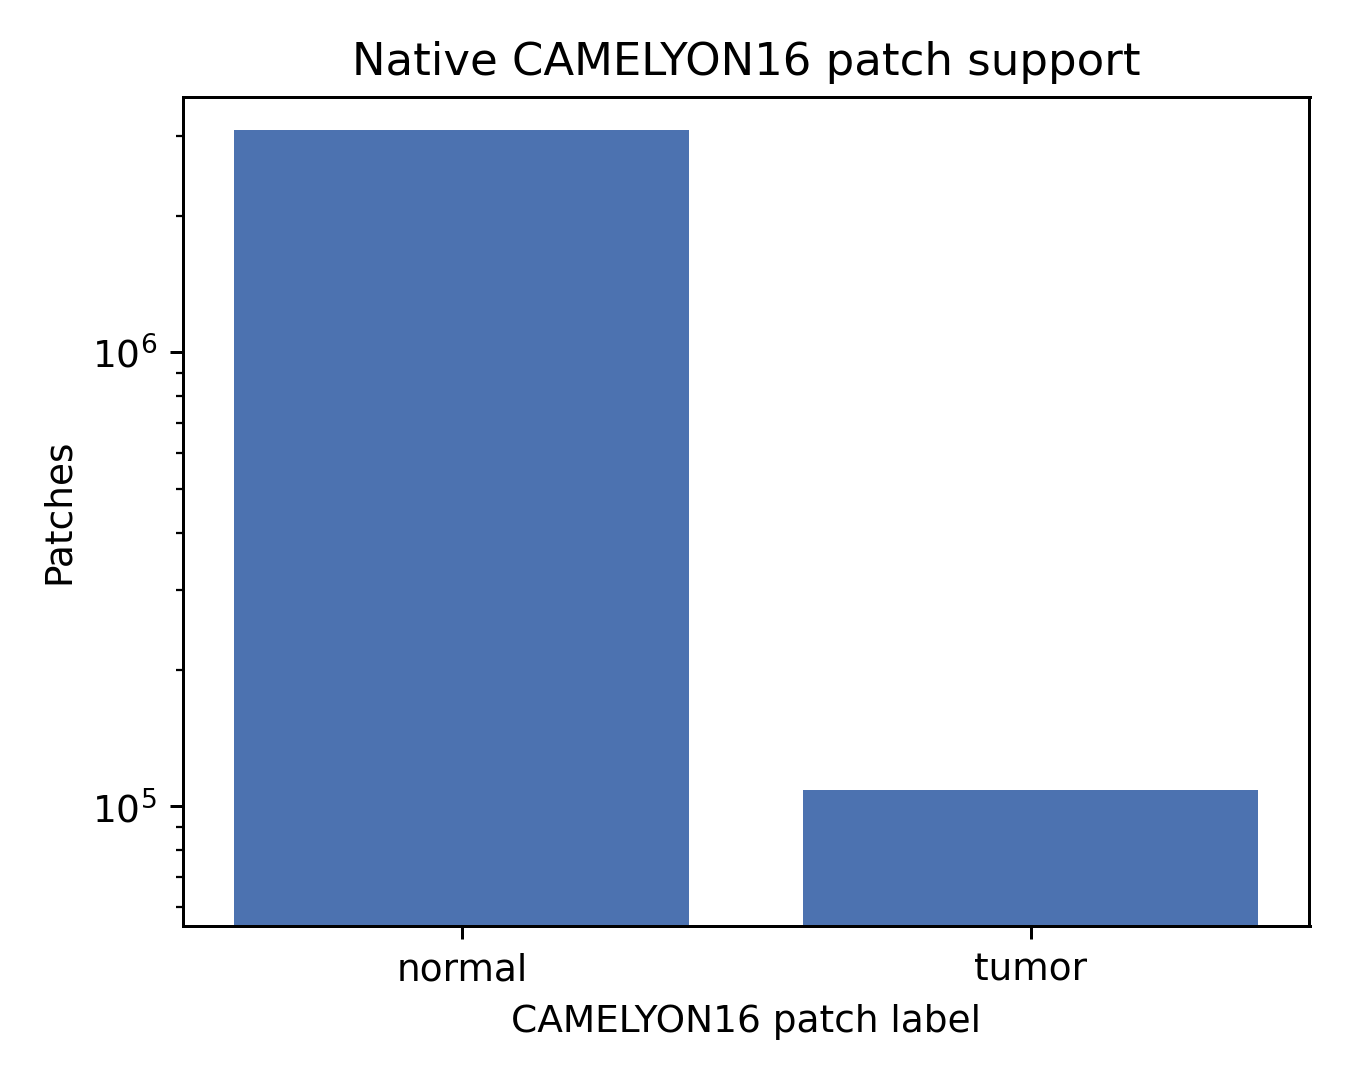
\includegraphics[width=0.6\linewidth]{camelyon16_class_distribution.png}%
  \caption{CAMELYON16 patch support by tumor/normal label after mask-based labelling
  (log scale). Tumor tiles are far scarcer than normal tiles.}
  \label{fig:camelyon16-dist}
\end{figure}

\subsection{TCGA-UT --- pan-cancer typing}
\label{sec:tcgaut}
TCGA-UT widens the lens from one organ to the whole body. It is derived from diagnostic WSIs in The
Cancer Genome Atlas (TCGA), a pan-cancer resource linking molecular and clinical data with large
image collections \citep{tomczak2015reviewThe}. The TCGA-UT release turns this slide archive into a
computational-pathology dataset by cropping H\&E tumour patches from pathologist-selected uniform
tumour regions: \num{1608060} RGB patches of $256\times256$ pixels from \num{8736} diagnostic slides,
across \num{32} cancer types \citep{komura2022universalEncoding}. These patches are not tiled here but
supplied by the dataset authors: for each slide at least three uniform tumour regions were delineated
as polygons by trained pathologists, and crops spanning six field-of-view sizes, from
$128\times128$ to $256\times256$~$\mu$m, were taken from them and resized to $256\times256$ pixels,
which puts their effective resolution at \num{0.5}--\num{1.0}~$\mu$m/px \citep{komura2022universalEncoding}.
No tissue-foreground filter is applied, the regions already being curated tumour. Every patch carries
the cancer-type label of the slide it was cropped from, so the patches are themselves labelled samples --- the unit
of patch-level classification --- while their slide identities also allow grouping into slide-level
bags. The labels are cancer types, not dense pixel masks or cell-level annotations, so the diagnostic
question is \emph{what cancer is it?}, a nominal classification across 32 cancer types.

The largest class is glioblastoma multiforme (GBM; \num{792} slides) and the smallest is diffuse
large B-cell lymphoma (DLBC; \num{28} slides), with the remaining types spread across a gradually
declining tail (Table~\ref{tab:tcgaut-summary}, Figure~\ref{fig:tcgaut-dist}).

\begin{table}[ht]
  \centering
  \begin{minipage}{0.30\linewidth}
    \centering
    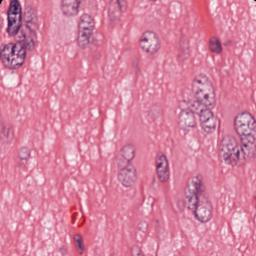
\includegraphics[width=\linewidth]{tcga_ut_example_patch.jpg}%
  \end{minipage}
  \hfill
  \begin{minipage}{0.64\linewidth}
    \centering
    \small
    \begin{tabular}{ll}
      \toprule
      Property & Value\\
      \midrule
      Cancer-type labels & \num{32}\\
      Diagnostic slides & \num{8736}\\
      Author-supplied patches & \num{1608060} of $256\times256$\\
      Largest class & Glioblastoma (GBM), \num{792} slides\\
      Smallest class & B-cell lymphoma (DLBC), \num{28} slides\\
      \bottomrule
    \end{tabular}
  \end{minipage}
  \caption{TCGA-UT dataset properties, alongside an example $256\times256$ H\&E tumor patch. Every
  patch inherits its slide's cancer-type label, so both regimes use the same label vocabulary;
  patch-level class proportions additionally depend on how many patches each slide contributes.}
  \label{tab:tcgaut-summary}
\end{table}

\begin{figure}[ht]
  \centering
  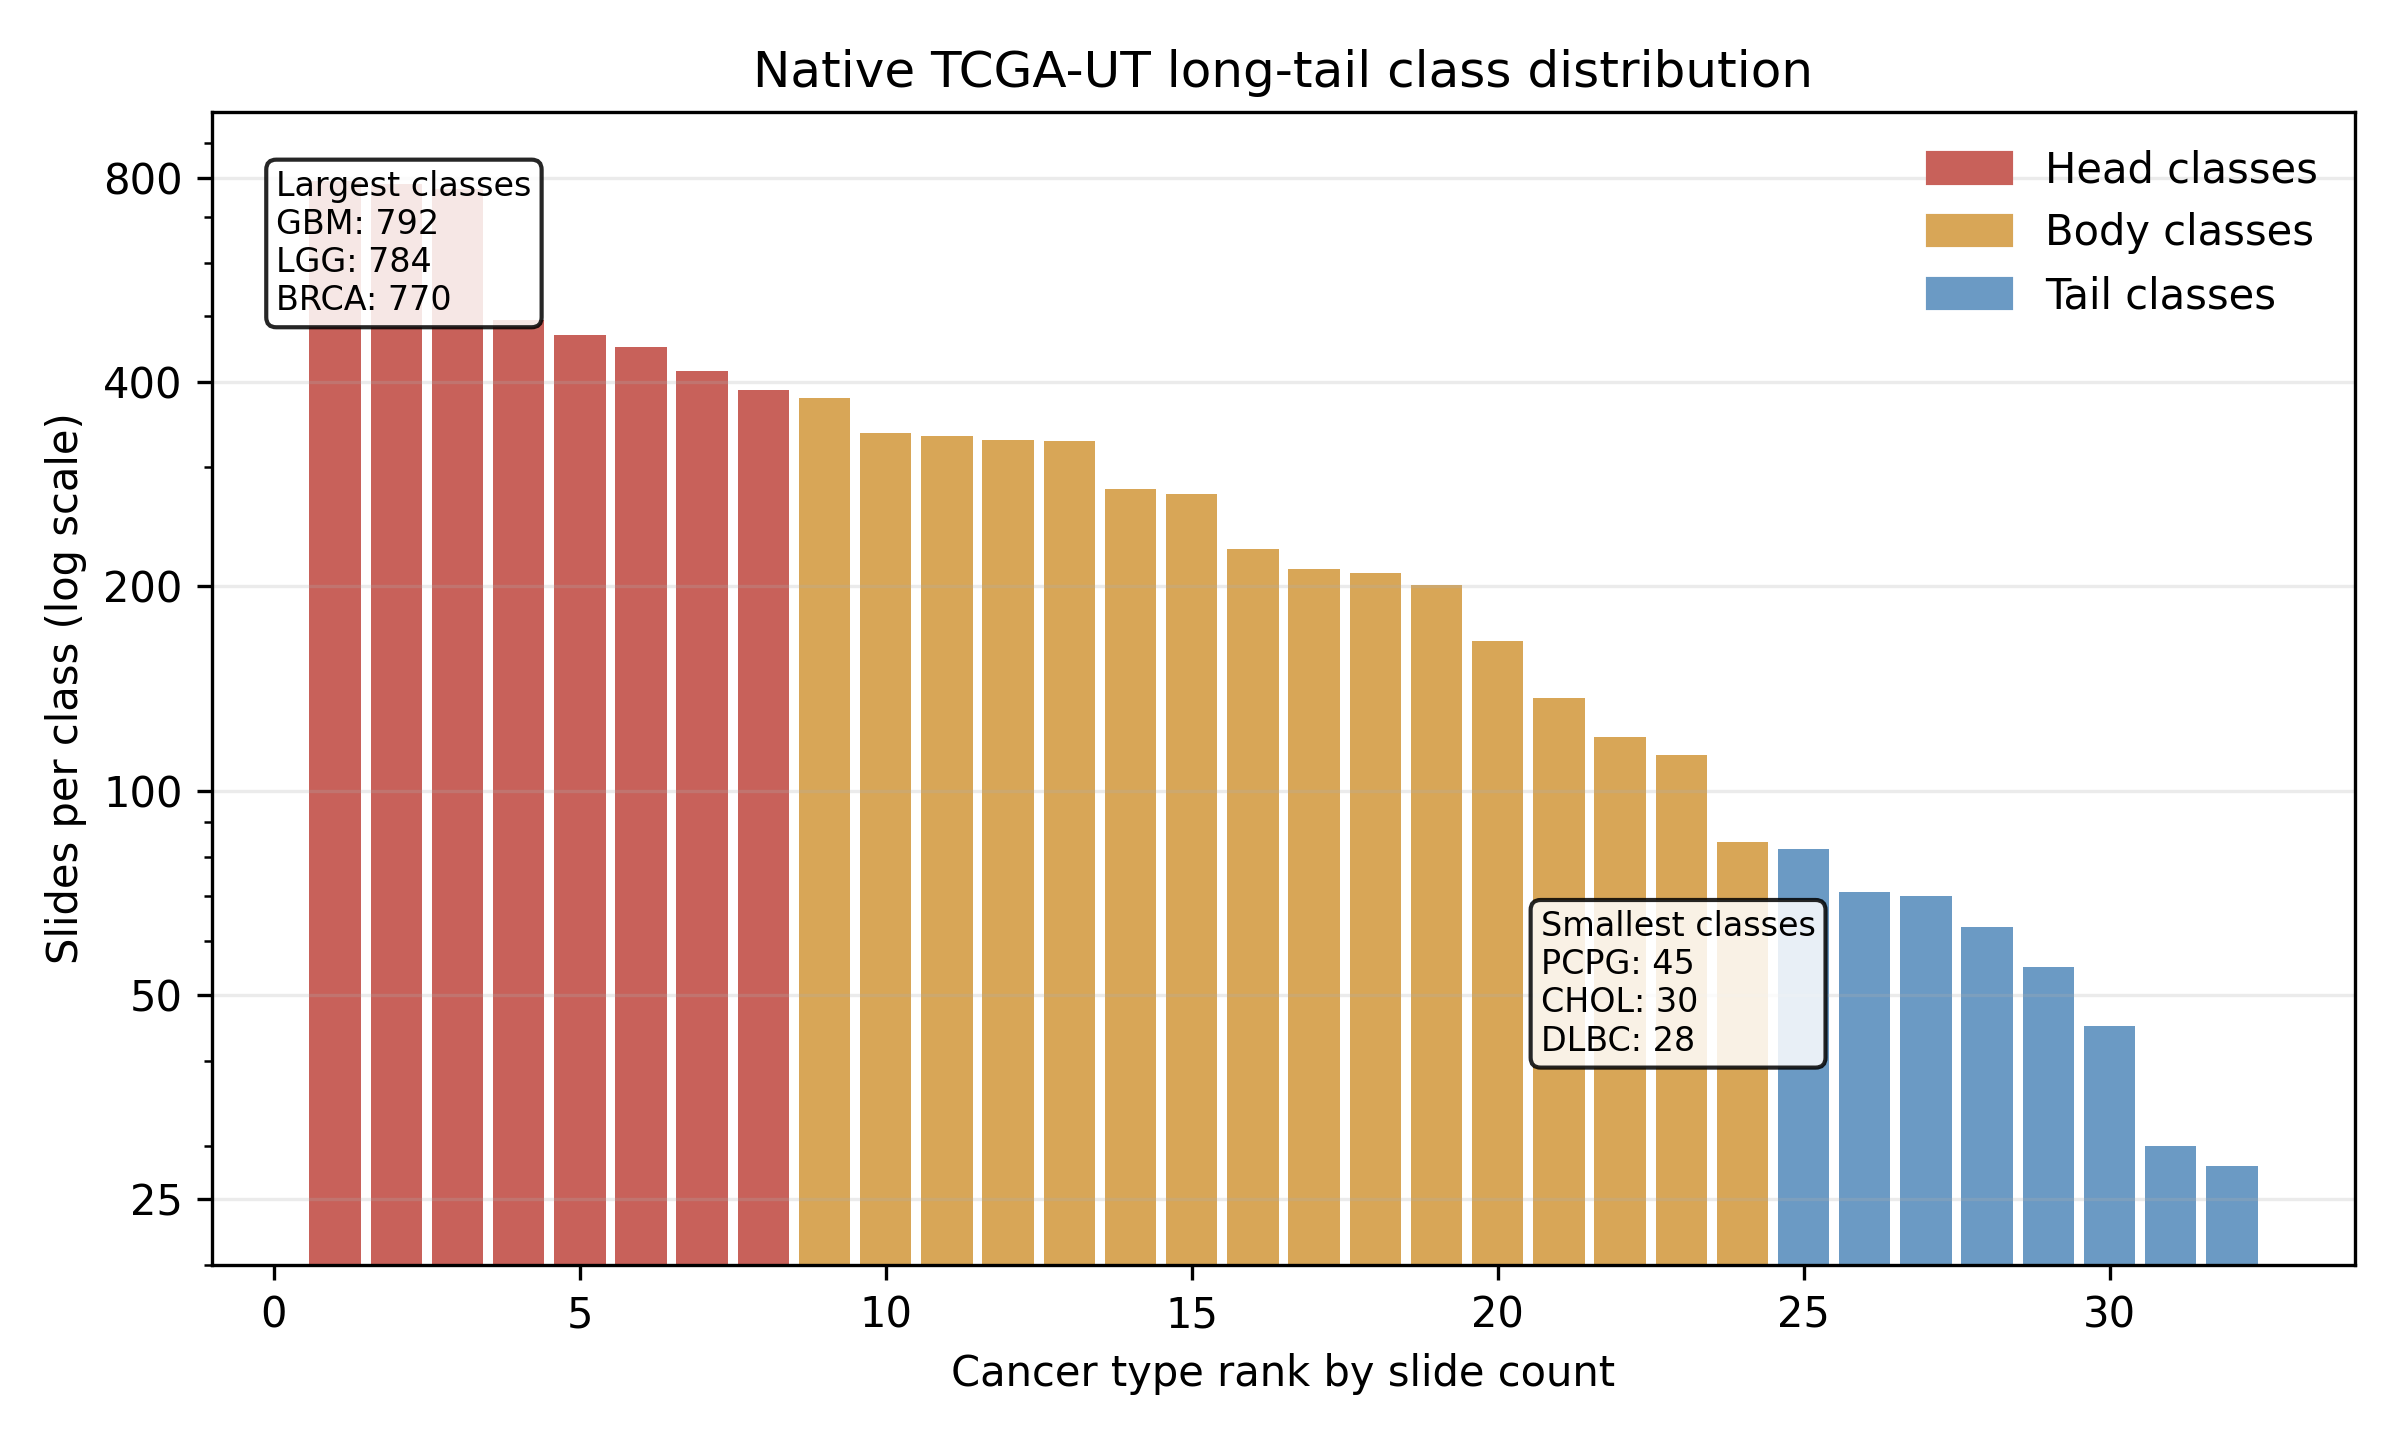
\includegraphics[width=0.86\linewidth]{tcga_ut_class_distribution.png}%
  \caption{TCGA-UT slide support by cancer-type rank, declining gradually across the \num{32}
  classes from GBM at the head to DLBC at the tail.}
  \label{fig:tcgaut-dist}
\end{figure}

\subsection{BRACS --- breast-lesion subtyping}
\label{sec:bracs}
BRACS narrows back to a single organ but sharpens the question from \emph{which cancer} to
\emph{how abnormal is this tissue}. It is an H\&E breast-pathology dataset of \num{547} WSIs from
\num{189} patients, with \num{4539} regions of interest (ROIs) drawn on \num{387} of those WSIs from
\num{151} patients. Three board-certified pathologists annotated both levels by consensus
\citep{brancati2022bracs}. The labels form three lesion types---benign, atypical, and
malignant---refined into seven subtypes: normal (N), pathological benign (PB), usual ductal
hyperplasia (UDH), flat epithelial atypia (FEA), atypical ductal hyperplasia (ADH), ductal carcinoma
in situ (DCIS), and invasive carcinoma (IC).

The patch regime uses the ROI annotations. A single slide may contain ROIs of several subtypes, and
each patch inherits the label of the particular ROI from which it is cut. The supplied ROI crops are
at the slides' native \num{0.25}~$\mu$m/px (\num{40}x) resolution and are gridded into non-overlapping
$256\times256$ tiles without a tissue-foreground filter because the crops already delimit tissue.
This yields \num{278028} labelled patches; \num{16} ROIs are too small to supply one complete tile.

The WSI regime instead uses the official single label assigned to each complete slide: the most
aggressive subtype detected by the pathologists. It therefore includes the \num{160} WSIs without
released ROIs and uses the full \num{547}-WSI, \num{189}-patient cohort. The official subtype counts
are N \num{44}, PB \num{147}, UDH \num{74}, FEA \num{41}, ADH \num{48}, DCIS \num{61}, and IC
\num{132}. Full WSIs are sampled at \num{20}x into non-overlapping $256\times256$ patches and use the
same deterministic foreground stack as CAMELYON16: at least \num{10}\% Otsu foreground, grayscale
standard deviation of at least \num{8}, Canny edge evidence, and at least two tissue neighbours. No
per-slide cap is applied. Thus the ROI-patch and WSI regimes share a subtype vocabulary but not a
label assignment rule, cohort, or prediction target.

\begin{table}[ht]
  \centering
  \begin{minipage}{0.32\linewidth}
    \centering
    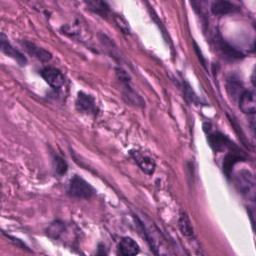
\includegraphics[width=\linewidth]{bracs_example_patch.jpg}%
  \end{minipage}
  \hfill
  \begin{minipage}{0.62\linewidth}
    \centering
    \small
    \begin{tabular}{ll}
      \toprule
      Property & Value\\
      \midrule
      Full WSI cohort & \num{547} WSIs / \num{189} patients\\
      ROI subset & \num{4539} ROIs / \num{387} WSIs / \num{151} patients\\
      ROI-derived patches & \num{278028}\\
      Subtype labels & N, PB, UDH, FEA, ADH, DCIS, IC\\
      \bottomrule
    \end{tabular}%
  \end{minipage}
  \caption{BRACS dataset properties, alongside an example $256\times256$ ROI patch. Patch labels are
  ROI specific, whereas each complete WSI has one official most-aggressive-lesion subtype.}
  \label{tab:bracs-summary}
\end{table}

\begin{figure}[ht]
  \centering
  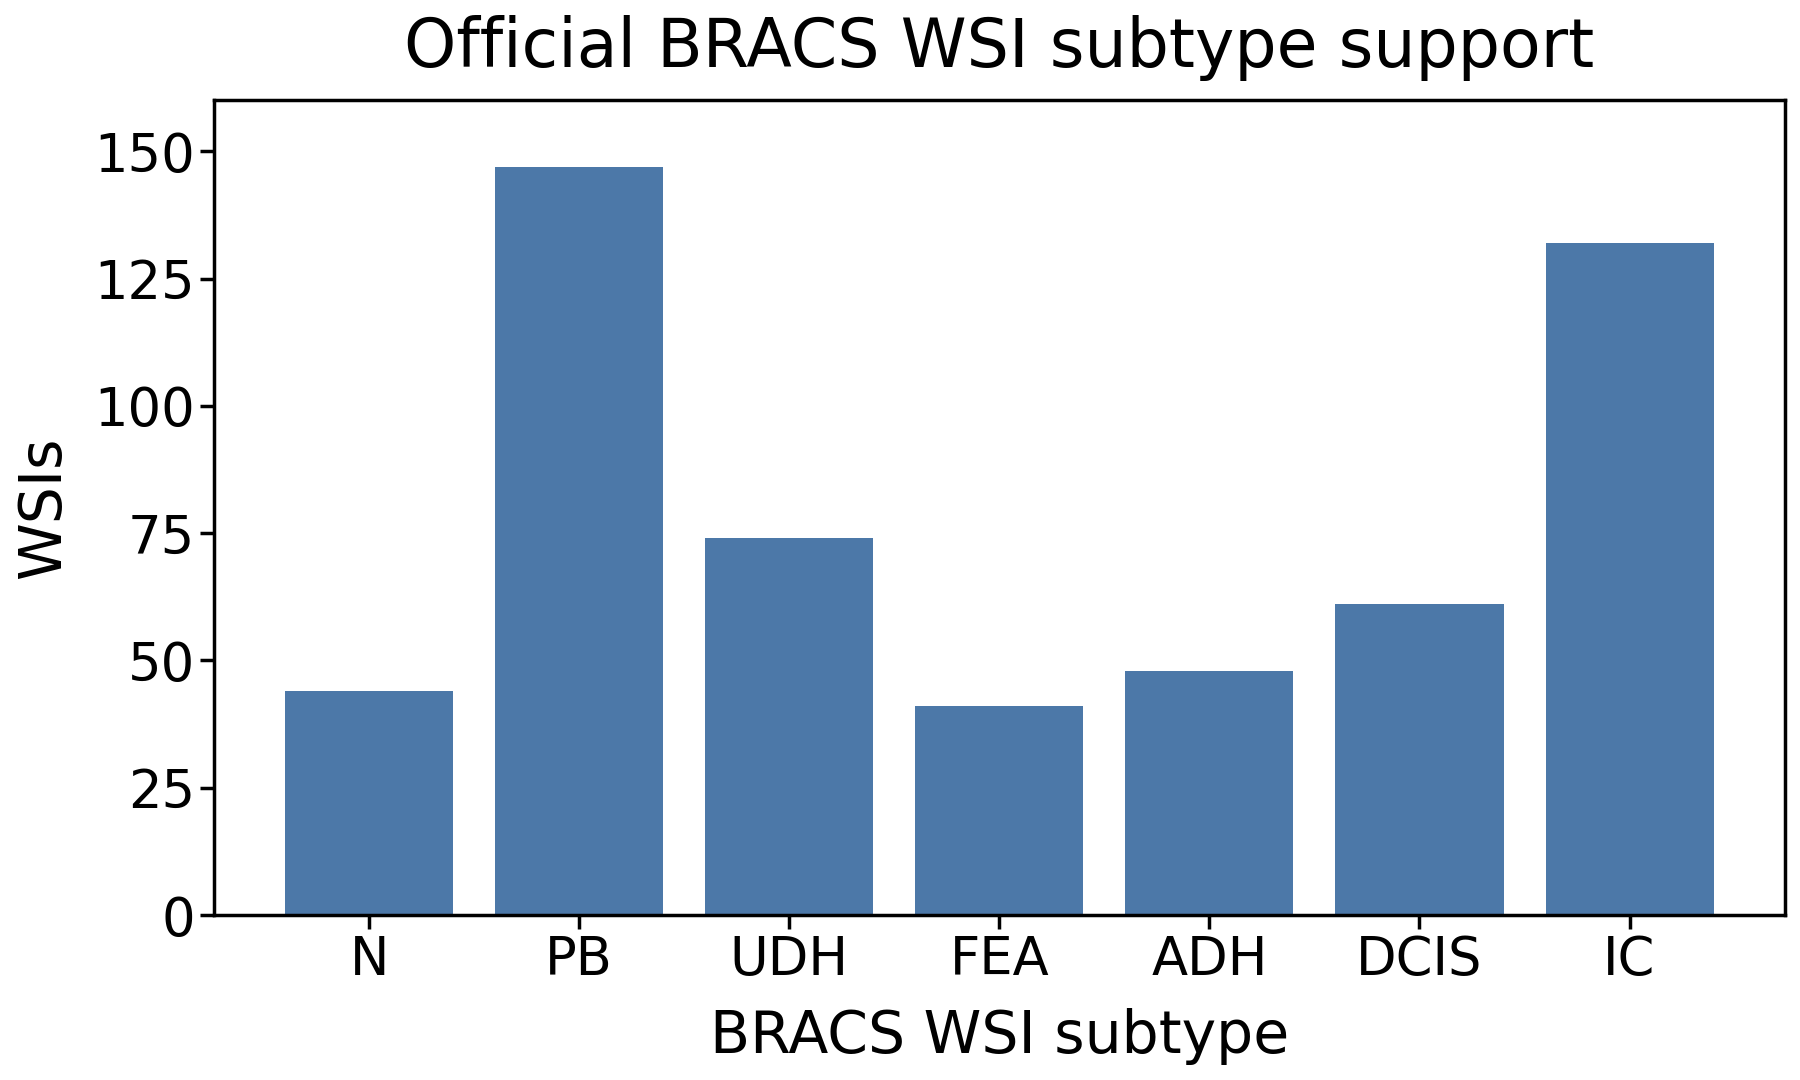
\includegraphics[width=0.72\linewidth]{bracs_class_distribution.png}%
  \caption{Official single-label BRACS WSI support by subtype across all \num{547} slides, from PB
  at the head to FEA at the tail.}
  \label{fig:bracs-dist}
\end{figure}

\subsection{PANDA --- prostate cancer grading}
\label{sec:panda}
PANDA (Prostate cANcer graDe Assessment) poses the most nuanced question --- \emph{how aggressive is
the cancer?} --- as an ordinal grading problem. It is an H\&E dataset of prostate core-needle biopsies
assembled for automated Gleason grading and the largest public cohort of its kind, with \num{10616}
whole-slide biopsies \citep{bulten2022panda}. Gleason grading describes prostate-cancer severity from
glandular growth patterns; pathologists summarise the dominant and secondary malignant patterns into
ordinal ISUP Grade Groups, where higher groups indicate more aggressive morphology. Here grade
\num{0} marks benign tissue and grades \num{1}--\num{5} are the ordered ISUP cancer groups.

PANDA differs from the other three along every axis a generality check exercises: a third organ
(prostate), an ordinal rather than nominal or binary label, and a built-in source of heterogeneity,
because the slides come from two institutions --- Radboud University Medical Center and Karolinska
Institute --- that differ in staining, scanning, and annotation convention, and grade differently
(Karolinska biopsies concentrate at low grades, Radboud spread more evenly). Across the full cohort of
\num{10616} biopsies (Karolinska \num{5456}, Radboud \num{5160}), the ISUP distribution runs from
ISUP\,0 (\num{2892} biopsies) at the head to ISUP\,5 (\num{1224}) at the tail --- a mild
${\approx}\num{2.4}{:}1$ slide-level imbalance.

Each biopsy is read at level~0, its native full resolution, divided into $256\times256$ tiles,
and a luminance foreground filter keeps a tile when at least \num{35}\% of its pixels are tissue, a
pixel counting as tissue when its mean RGB value is below \num{210}, discarding glass and
background. No per-slide cap is applied, so the counts reflect each biopsy's full available
tissue. PANDA's masks additionally support a provider-consistent binary cancer/benign tile label
--- the only labelling the two institutions share --- formed by collapsing the provider-specific
mask codes and calling a tile \emph{cancer} when at least half of its mask cell
carries a cancer value. Over the \num{10514} masked biopsies that yield labelled tissue this gives
\num{3702544} benign against \num{803785} cancer tiles, so the same biopsies furnish both an ordinal
slide-level grading target and a binary tile-level detection target (Table~\ref{tab:panda-summary},
Figure~\ref{fig:panda-dist}).

PANDA carries two independent label sources at two granularities: a slide-level ordinal ISUP grade,
which summarises the whole biopsy and cannot be assigned to a single tile, and pixel masks that yield
a per-tile cancer/benign label. CAMELYON16 likewise changes granularity, from local tumour tissue to
the slide's metastasis status. BRACS changes from the subtype of a selected ROI to the official most
aggressive subtype on the complete WSI. Only TCGA-UT uses the same cancer-type target in both regimes;
there, the prediction unit changes but the target does not.

\begin{table}[ht]
  \centering
  \begin{minipage}{0.32\linewidth}
    \centering
    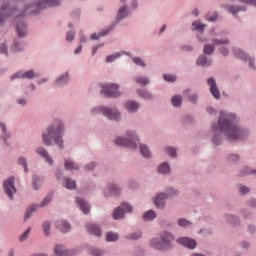
\includegraphics[width=\linewidth]{panda_example_patch.jpg}%
  \end{minipage}
  \hfill
  \begin{minipage}{0.62\linewidth}
    \centering
    \small
    \begin{tabular}{ll}
      \toprule
      Property & Value\\
      \midrule
      WSIs (biopsies) & \num{10616}\\
      Patch-labelled WSIs & \num{10514}\\
      Slide labels / patch labels & ISUP 0--5 / benign, cancer\\
      Eligible patches (benign / cancer) & \num{3702544} / \num{803785}\\
      \bottomrule
    \end{tabular}%
  \end{minipage}
  \caption{PANDA dataset properties, alongside an example $256\times256$ cancer patch (ISUP\,5
  Radboud biopsy). Unlike the other datasets, patch and slide labels define different tasks: binary
  cancer detection and six-class ISUP grading, respectively.}
  \label{tab:panda-summary}
\end{table}

\begin{figure}[ht]
  \centering
  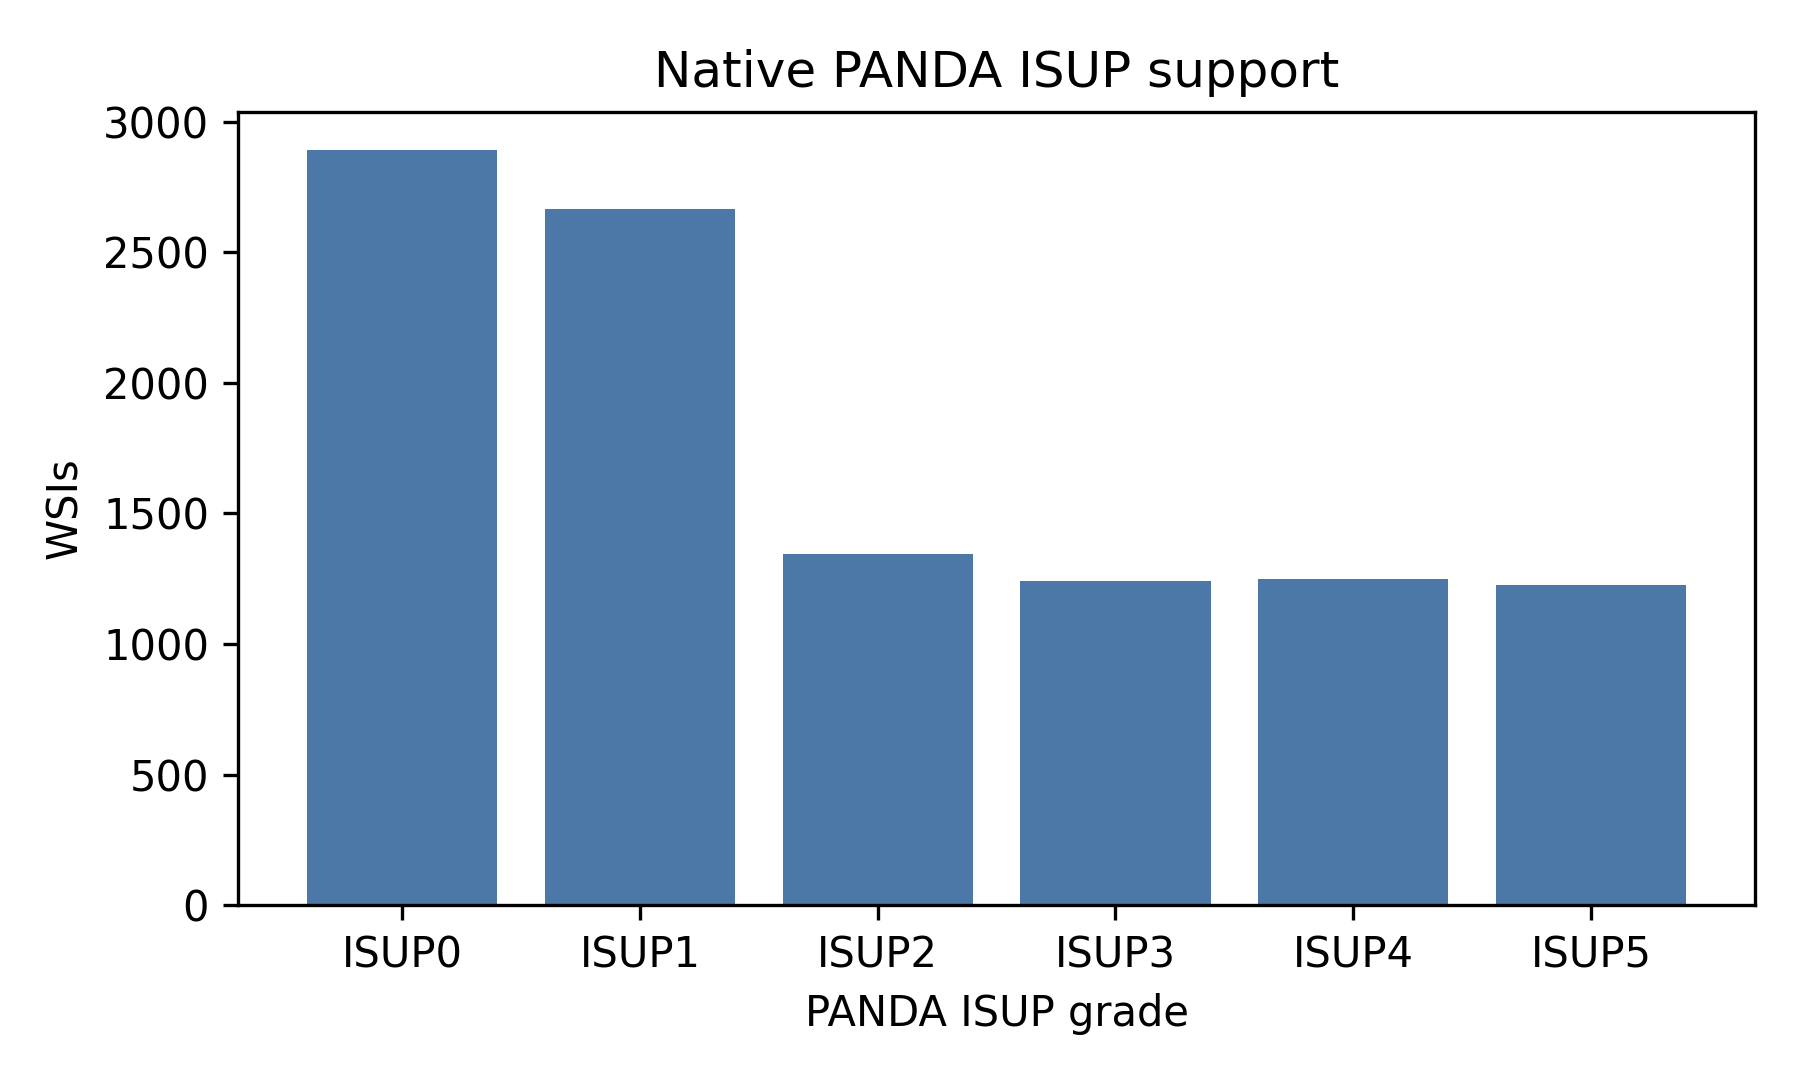
\includegraphics[width=0.72\linewidth]{panda_class_distribution.png}%
  \caption{PANDA WSI support by six-class ISUP grade across the full \num{10616}-biopsy cohort, from
  ISUP\,0 at the head to ISUP\,5 at the tail.}
  \label{fig:panda-dist}
\end{figure}

\section{Summary}
\label{sec:summary}
This report introduced the computational-pathology pipeline --- from a stained glass slide to a
gigapixel whole-slide image, patching, weakly supervised multiple-instance learning, and frozen
foundation-model features --- and the four H\&E datasets it covers, presented as a
progression of diagnostic questions from CAMELYON16 detection through TCGA-UT typing and BRACS
subtyping to PANDA grading, each with its organ, label type, annotation form, example patch, and
class distribution.

\clearpage
\bibliographystyle{plainnat}
\bibliography{references}

\end{document}
